\documentclass{article}
\usepackage{graphicx}
\begin{document}

Kubitschek e Chekskubit são os dois cachorros vira-latas que compõem a dupla de notórios criminosos procurados pelos seus terríveis, impiedosos, horripilantes, amedrontadores e imperdoáveis crimes cometidos nos arredores da UFOP (Universidade Fictícia do Oeste do Paraná). Entre os crimes realizados pela dupla, o que mais tomou notoriedade foi o de cometer, mais de uma vez, o ato terrorista de comer restos de refeições ofertados pelos alunos do campus, que, caso contrário, seriam despejados no lixo.

Diante desse crime abominável, um dos setores da UFOP, o RUF (Restaurante Universitário Fictício), entrou em contato com as autoridades e cobrou que tomassem providências contra esses bandidos perigosíssimos. Em resposta, a polícia iniciou uma campanha para capturá-los, imprimindo panfletos de "procurado" com recompensas para quem os entregasse.

Cada um dos panfletos contém as seguintes proporções:
\begin{itemize}
    \item O panfleto de Kubitschek tem proporção de altura/largura igual a 5:3.
    \item O panfleto de Chekskubit tem proporção de altura/largura igual a 3:2.
\end{itemize}

Você foi contratado para ajudar a polícia a descobrir quantos panfletos de Kubitschek e Chekskubit podem ser impressos em uma cartolina retangular de dimensões $X:Y$, de modo que a diferença entre a quantidade de panfletos de cada um dos criminosos não seja maior que 1 (ou seja, a quantidade de panfletos de Kubitschek e Chekskubit deve ser a mais equilibrada possível). Além disso, cada panfleto, seja de Kubitschek ou de Chekskubit, deve ter uma área igual a 5\% da área total da cartolina.

\subsection*{Ilustração dos panfletos}

\begin{center}
    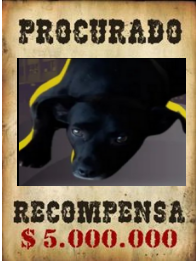
\includegraphics[width=0.3\textwidth]{forasdalei/kubitschek.png}
    \hspace{1cm}
    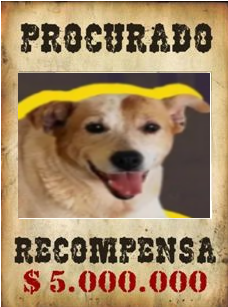
\includegraphics[width=0.3\textwidth]{forasdalei/chekskubit.png}
\end{center}

\subsection*{Entrada}
A entrada consiste de dois inteiros $X$ e $Y$ representando as dimensões da cartolina $(1 \leq X, Y \leq 10^9)$.

\subsection*{Saída}
A saída deve consistir de um único número inteiro representando a quantidade máxima de panfletos de Kubitschek e Chekskubit que podem ser impressos na cartolina.

\end{document}
